\chapter{测试自动生成}

    现在, 有了OpenAPI规约语言描述的API行为文档, 和场景模型, 接下来的任务就是生成并执行测试了. 测试的生成有两个层次: 一个是为单次API请求生成请求数据(即输入数据), 一个是将单个请求串联起来生成API执行序列作为测试用例.
    
    \section{构建与实现}
        场景模型抽象了API的使用场景, 并为生成高效的测试用例提供了必需的知识. 目前, 场景模型需要手工进行构建与设计, 然后才能自动生成与执行测试用例. 未来, 将进一步探索如何从自然语言描述和日志文件中进行自动化场景生成
        
        场景模型使用与OpenAPI规约语言类似的规约语言描述, 并用YAML格式记录.
        
        在具体实现上, 合法输入(包括输入依赖), 合法响应(包括输出断言), 转移条件的定义($in_q$, $out_q$, $f_d$, $f_a$, $x \in Sigma$)的定义有多种来源:
        
        \label{sec:set_define}
        \begin{itemize}
            \item JSON模式(JSON Schema)\footnote{https://tools.ietf.org/html/draft-wright-json-schema-validation-00}.\\
            JSON模式被用于结构化JSON数据的验证. 对于一个JSON模式定义而言, 通过验证的数据构成了一个固定集合. 当所需集合不依赖于其他状态(即上下文)时, 便可以使用JSON模式定义. 在使用OpenAPI描述的API脚本文档中, 均采用这种方法定义合法输入和合法响应. 场景模型中的状态定义如果关联了一个API服务端点, 则默认将此API的脚本文档中的合法输入, 合法响应的定义作为该状态的合法输入, 合法响应定义. 此外, 由于输入依赖和输出断言需要定义依赖上下文的函数($f_d$, $f_a$), 一般不使用JSON模式定义. 
            
            \item 自定义校验函数.\\
            本文的工具原型支持可扩展插件. 用户可以编写并引入校验函数, 校验函数接受数据作为输入, 判定数据是否满足条件. 因此, 满足条件的数据构成了一个集合. 这种定义方式只能在合法响应(包括输出断言)和转移条件的定义中使用, 而不能用于定义合法输入, 因为定义合法输入时还需要在定义的集合中采样, 而只判定是否属于某集合的函数显然不具备此功能.
            
            \item 自定义生成函数.\\
            用户可以编写并引入生成函数, 生成函数要求随机返回一个在其隐式定义的集合内的元素. 生成函数可以用于定义合法输入(包括输入依赖), 这是因为测试时只需要获得满足条件的数据即可. 但是, 由于生成函数不能判定某个数据是否属于其定义的集合, 也不能获取其定义集合的所有元素. 所以它不能用于定义合法响应和转移条件.
        \end{itemize}
        
    \section{请求数据生成}
        \label{sec:req_data_gen}
    
        请求数据的生成, 就是在合法请求数据集合中的随机采样. \ref{sec:set_define}小节总结了目前支持的集合定义方法: 在定义合法输入时, 有JSON模式和自定义生成函数两种定义方法.
        
        当合法输入使用JSON模式定义时, 由于每个数据结构都属于JSON模式定义的基本类型之一, 因此, 分类讨论为每个基本类型设计采样策略即可. 此外, 对于一些特殊子类型如日期、时间、二进制串等, 本文定义了特殊采样策略. 具体策略见表\ref{tab:schemagen}. 特别地, 当多个条件均满足时, 则合理结合多个策略生成.
        
        \begin{table}[!htb]
            \centering
            \begin{tabular}{rll}
                \toprule
                类型 & 条件 & 策略 \\
                \midrule
                null & / & 返回元素\texttt{Null} \\
                \hline
                integer \& & 存在\texttt{multipleOf}域 & 从满足倍数关系的值空间中采样 \\
                \cline{2-3}
                float & 存在\texttt{enum}域 & 从定义的有限集合中采样 \\
                \cline{2-3}
                & 存在\texttt{MIN}或\texttt{MAX}域 & 从定义的区间中采样 \\
                \cline{2-3}
                & / & 在对应类型的整个区间中采样 \\
                \hline
                boolean & 存在\texttt{enum}域 & 从定义的有限集合中采样 \\
                \cline{2-3}
                & / & 使用伯努利分布($p=0.5$) \\
                \hline
                string & 存在\texttt{regex}域 & 从正则表达式定义的模式中生成 \\
                \cline{2-3}
                & 存在\texttt{enum}域 & 从定义的有限集合中采样 \\
                \cline{2-3}
                & \texttt{format}域存在 & 先随机日期, \\
                & 且为\texttt{'date'} & 再以RFC3339的full-date格式表示 \\
                \cline{2-3}
                & \texttt{format}域存在 & 先随机日期时间, \\
                & 且为\texttt{'datetime'} & 再以RFC3339的date-time格式表示 \\
                \cline{2-3}
                & \texttt{format}域存在 & \multirow{2}{*}{随机二进制串, 以\texttt{bytes}格式返回} \\
                & 且为\texttt{'binary'} &  \\
                \cline{2-3}
                & 存在\texttt{minLength} & 先从指定长度区间随机长度值, \\
                & 或\texttt{maxLength}域 & 再随机生成字符串 \\
                \cline{2-3}
                & \multirow{2}{*}{/} & 先随机确定长度值(默认不超过255),\\
                & & 再随机生成字符串 \\
                \hline
                array & 存在\texttt{maxItems} & 先从指定区间随机列表长度,\\
                & 或\texttt{minItems}域 & 再随机递归生成各元素 \\
                \cline{2-3}
                & \multirow{2}{*}{/} & 先随机确定列表长度,\\
                & & 再随机递归生成各元素 \\
                \hline
                object & / & 递归生成各成员 \\
                \bottomrule
            \end{tabular}
            \caption{从JSON模式生成请求数据. 依据基本类型和条件分类讨论, 采取不同策略.}
            \label{tab:schemagen}
        \end{table}
        
        当合法输入使用自定义生成函数定义时, 由于函数期望的返回值就是其隐式定义的集合的采样, 故直接将返回值作为请求数据即可.
        
    \section{执行序列生成}
        如果以自动机的视角审视场景模型, 那么它所定义的仍然是合法串的集合以及它们的概率分布. 由于每个自动机的状态可以与一个API服务端点关联, 所以产生的串也可以对应于API的请求/执行序列. 在进行web API测试时, 一个这样的包含具体请求数据的序列, 即是一个测试用例.
        
        因此, 执行序列生成算法的基本思想, 就是根据场景模型定义的概率分布生成可以被其接受的串. 相比看似相近的概率图模型和马尔科夫模型, 场景模型中转移到某一状态不仅仅由当前状态和概率分布决定. 由于每项转移是否可用取决于关联的API服务端点的响应结果, 而API服务端点的响应结果取决于输入的请求数据, 请求数据的生成过程依赖整个当前序列, 故状态转移还可以与之前的所有状态均相关. 因此, 场景模型的表达能力要强于仅与当前状态和概率分布相关的概率图模型与马尔科夫模型.
        
        执行序列生成算法的大体流程如算法\ref{algo:seqgen}所示.
        
        在算法\ref{algo:seqgen}中, 首先, 根据初始状态概率分布函数$I_{\mathcal{A}}$随机选择初始状态. \texttt{RandomChoice()}函数接受两个列表作为参数, 分别表示候选元素和每个元素的概率权重, 它按照权重随机抽取一个元素作为返回值, 故\texttt{RandomChoice(}$Q_{\mathcal{A}}$\texttt{,}$I_{\mathcal{A}}$\texttt{)}返回随机选择的初始状态. 然后, 算法在自动机上进行遍历. 每一步中, 使用$current$记录当前所处状态, 请求数据和响应数据等上下文信息. $r$是存储整个序列的上下文信息的总列表. 如果当前状态与一个API服务端点相关联, 算法将遍历请求数据的各个参数定义, 并从数据依赖定义或合法集合定义中随机生成出参数. 之后, 算法发送请求并解析响应体. 解析完成后, 算法扫描响应的各个域, 根据断言定义或合法集合定义进行验证, 如果验证不通过, 算法终止. 最后, 算法根据终止概率分布函数$F_{\mathcal{A}}$进行概率终止, 若未终止, 则根据响应和转移概率函数$P_{\mathcal{A}}$随机选择下一状态, 进入下一步.
        
        当算法结束时, 返回的值包括执行序列$r$和终止原因$T$, 其中终止原因$T$详细记录了跳出算法循环的位置和具体信息, 便于发现被测系统故障时进行修复.
        
        从描述中可以看出, 算法结合了执行序列的生成和执行过程, 并且生成过程实时受执行结果(即API响应)的反馈影响. 序列生成是动态的, 这使预处理相关的加速和优化变得困难, 但也使生成的序列更为灵活, 更为贴近实际使用场景.
        
        \begin{algorithm}
          	\scriptsize
          	
            \caption{API执行序列生成算法}
          	
            \KwIn{$Spec$, $\mathcal{A}$} 
            \tcp{输入: API定义脚本和场景模型脚本}
            \tcp{场景模型$\mathcal{A} := <Q_{\mathcal{A}}, \Sigma, \sigma_{\mathcal{A}}, I_{\mathcal{A}}, F_{\mathcal{A}}, P_{\mathcal{A}}>$}
            \KwOut{$r$, $T$}
            \tcp{输出: 执行序列和终止原因}
            $q$ $\gets$ RandomChoice($Q_{\mathcal{A}}$, $I_{\mathcal{A}}$)\;
            \tcp{根据初始状态概率分布函数随机初始状态$q := <t_q, in_q, out_q, d_q, a_q>$}
            $current$ $\gets$ $EmptyMap$\;
            $current.state$ $\gets$ $q$\;
            $r$ $\gets$ $EmptyList$\;
            $stop$ $\gets$ $false$\;
            \While {$\neg stop$} {
            	$i$ $\gets$ $EmptyMap$\;
                $o$ $\gets$ $EmptyMap$\;
            	\If(\tcp*[h]{$q$有关联的API服务端点}) {$t_q \neq empty$}{
                	\ForEach(\tcp*[h]{遍历处理所有请求参数}) {$param$ in $t_q.params$} {
                    	\If(\tcp*[h]{当前参数$param$有数据依赖, 则从依赖生成请求数据}) {$d_q.param \neq Null$} {
                        	$d$ $\gets$ $d_q.param$\;
                            \tcp{数据依赖$d := <q_d, index_d, f_d>$}
                            $q'$ $\gets$ PickDependee($r$, $q_d$, $index_d$)\;
                            $i.param$ $\gets$ RandomFromSet($f_d(i_{q'}, o_{q'})$)\;
                        } \Else(\tcp*[h]{当前参数$param$无数据依赖, 则默认从合法请求集合中生成请求数据}) {
                        	$i.param$ $\gets$ RandomFromSet($in_q.param$)\;
                        }
                    }
                    $o$ $\gets$ Request($Spec.t_q$, $i$)\;
                    \tcp{发送请求, 并解析返回的响应}
                    $current.i$ $\gets$ $i$\;
                    $current.o$ $\gets$ $o$\;
                    \If(\tcp*[h]{请求失败}) {RequestFail($o$)} {
                    	$T$ $\gets$ ``Request Fail''\;
                        $stop$ $\gets$ $true$\;
                    } \Else(\tcp*[h]{请求成功}) {
                    	\ForEach(\tcp*[h]{遍历返回的响应的各个域}) {$field$ in $Spec.t_q.fields$} {
                        	\If(\tcp*[h]{响应的$field$域有断言定义, 则验证是否满足断言}) {$a_q.field \neq Null$} {
                            	$a$ $\gets$ $a_q.field$\;
                                \tcp{响应断言$a := <q_a, index_a, f_a>$}
                                $q'$ $\gets$ PickDependee($r$, $q_a$, $index_a$)\;
                                \If {$o.field \notin f_a(i_{q'}, o_{q'})$} {
                                	$T$ $\gets$ ``Response Assert Fail''\;
                                    $stop$ $\gets$ $true$\;
                                }
                            } \Else(\tcp*[h]{响应的$field$域无断言定义, 则默认直接验证是否是合法响应}) {
                            	\If {$o.field \notin out_q.field$} {
                                	$T$ $\gets$ ``Response Illegal Fail''\;
                                    $stop$ $\gets$ $true$\;
                                }
                            }
                        }
                    }
                }
                $r$.append($current$)\;
                \If {$\neg stop$} {
                	$\chi$ $\gets$ RandomNumber($U(0,1)$)\;
                    \If(\tcp*[h]{依照终止概率分布函数决定是否终止执行}) {$\chi \le F_{\mathcal{A}}(q)$} {
                    	$T$ $\gets$ ``Final State''\;
                        $stop$ $\gets$ $true$\;
                    }
                }
            	\If(\tcp*[h]{继续执行, 依照转移概率分布函数选择转移边}) {$\neg stop$} {
                	$q$ $\gets$ RandomChoice($\sigma_{\mathcal{A}}(q,o)$, $P_{\mathcal{A}}(q,o)$)\;
                    $current$ $\gets$ $EmptyMap$\;
                    $current.state$ $\gets$ $q$\;
                }
            }
            \Return {$r$, $T$}

            \label{algo:seqgen}
          \end{algorithm}
        
    \section{启发式执行序列生成}
        除了以上提出的算法, 本文亦探索了启发式的执行序列生成. 启发式的改进主要在转移边的选择方面. 在以上算法中, 转移边的选择严格按照定义的概率权值, 然而, 在运行此算法多次以生成多个测试用例时, 为了提高测试覆盖率, 可以不必拘泥于定义的权值, 而进行一定的调整.
        
        在此场景模型中, 测试覆盖率常常与场景的状态覆盖率, 转移覆盖率, 以及综合路径覆盖率正相关. 一个基本的思想便是将这些覆盖率的提升期望加入考虑, 对提升这些覆盖率幅度较大的转移边增大选择概率.
        
        一种贪心策略是优先选择连接到未访问状态的转移边, 或直接选择未访问的转移边. 但是, 本文的实验发现, 由于场景模型目前采用人工设计, 包含的状态数和转移边数较少, 因此少量测试用例即可完全遍历, 故价值不大. 其他更复杂的转移很可能会有效, 如考虑连续状态序列或整体路径的覆盖率等, 这有待进一步实验证实.
        
        另一方面, 启发式改进的直接作用亦可能并不显著. 虽然不使用启发式算法时, 测试用例冗余度较高, 即单位用例覆盖率不够高. 但受益于全自动生成的过程, 同等时间下, 生成测试用例的数目很大, 这可在一定程度上弥补甚至逆转总覆盖率的劣势. 具体结论需要依据具体场景模型进行评估, 也是值得进一步探讨的问题.
    
    % extended version
    % \section{*启发式优化}
    %     \subsection{启发式执行序列生成}
    %     将上个小节移到本章来
    %     \subsection{启发式场景优化}
    %     不知道有冇时间做了

    \section{实验与评估}

        \label{sec:experiment}

        本工作的原型系统在三个实际的web API服务上进行了实验, 从四个方面评估了本文提出的场景模型和测试方法: 测试用例多样性, 测试覆盖率, 故障检测能力, 以及测试效率.
    
        \subsection{实验配置}
            实验选择的第一个被测系统为合作研究组开发的云对象存储服务(OSS)的系统原型(后文简称\textbf{OSS}). 此服务提供了33个web API接口, 并有较完整的使用文档. 测试时, 期望所有的API和功能点均业已实现完成.
            
            最近以来, 云对象存储服务(OSS)已经成为了流行的云存储服务形式. 许多大型云服务提供商均已提供云对象存储服务, 如亚马逊AWS\footnote{https://aws.amazon.com/s3}, IBM云\footnote{ https://console.bluemix.net/catalog/services/cloud-object-storage}和阿里云\footnote{ https://www.alibabacloud.com/product/oss}等. 在云对象存储服务中, 每个账号, 在每个服务器区域, 都可以有许多存储空间(bucket). 存储空间(bucket)与文件系统中的文件夹类似, 对象(object)与文件系统中的文件类似. 用户可以上传对象, 删除对象, 重命名对象, 创建符号链接等等. 每个对象都属于一个固定的存储空间.
            
            对于云对象存储服务, 本工作首先为这33个API编写了OpenAPI格式的API行为描述脚本. 然后, 设计了一些小型场景模型来检验每个API的基本功能. 在此之后, 设计了三个较大型的综合场景模型Scenario A(详见附录图\ref{fig:oss_scenario_A})、Scenario B(详见附录图\ref{fig:oss_scenario_B})、Scenario C(详见附录图\ref{fig:oss_scenario_C})以进行综合测试, 这三个场景均与实际使用场景较相似, 测试用例的生成与执行期望能够模拟实际部署后的高负载环境. 对于每个场景, 运行工具原型随机生成并执行了1,000个测试用例. 所有测试用例及其执行结果都被妥善保存. 后续分析时, 在所有测试用例上进行统计, 未进行任何遴选.
            
            第二个被测系统为阿里云的云服务器(ECS)服务(后文简称\textbf{ECS}), 阿里云是世界领先的云计算服务商, 淘宝等大型应用均依托阿里云提供计算支持. 
            
            本实验测试阿里云为普通用户提供的云计算实例租用服务, 相关接口共有26个, 均为web API, 并配有详细用户使用文档. 在此服务中, 用户可以租用实例, 退租实例, 获取实例运行状态, 启动实例, 关闭实例, 重启实例等等. 我们选择了其中8个web API, 编写了行为描述脚本, 然后设计了包含所有这8个web API的综合场景模型(详见附录图\ref{fig:ecs_scenario})进行测试. 一共随机生成并执行了100个测试用例, 所有测试用例在进行统计与分析时均纳入考虑.
            
            第三个被测系统是工业界合作团队提供的电子支付服务(后文简称\textbf{E-payment}). 本实验测试它的实时贷记API接口. 此API仅用于系统内部使用, 是微服务之间的通信接口, 因此使用LAN上的定制协议交互. 作为电子支付接口, 此服务拥有很高的可用率与很低的容错率要求. 同时, 它有多达20个参数. 由于模拟环境的缺失, 在本实验中, 暂未进行实际的调用与发送, 而是根据接口描述文档进行测试用例和请求数据的生成, 来验证生成的测试用例可以有效覆盖参数组合, 从而验证其在这类服务的测试上的可用性.
            
            对于E-payment服务, 实验中生成了巨量(超过两百万个)的测试用例, 并计算了这些测试用例对于参数组合的覆盖率. 这种方式不仅仅评估了测试用例的覆盖率, 也检验了工具原型的鲁棒性和性能. 使用的场景主要进行基于数据分区的请求参数生成和参数合成操作, 详见附录图\ref{fig:epayment_scenario}.
            
        \subsection{测试用例多样性}
            富有多样性的测试用例是本文测试方法追求的目标之一. 多样性保证了测试用例集构成的测试套件具有较高的覆盖率和较低的冗余度. 另一方面, 使用被测系统的用户形形色色, 实际的系统负载也十分富有多样性, 因此, 测试用例富有多样性, 在某种程度上也能说明生成它们的测试场景模型可以很好地表达使用场景.
            
            \begin{figure}[!htb]
                \begin{minipage}{0.5\textwidth}
                    \centering
                    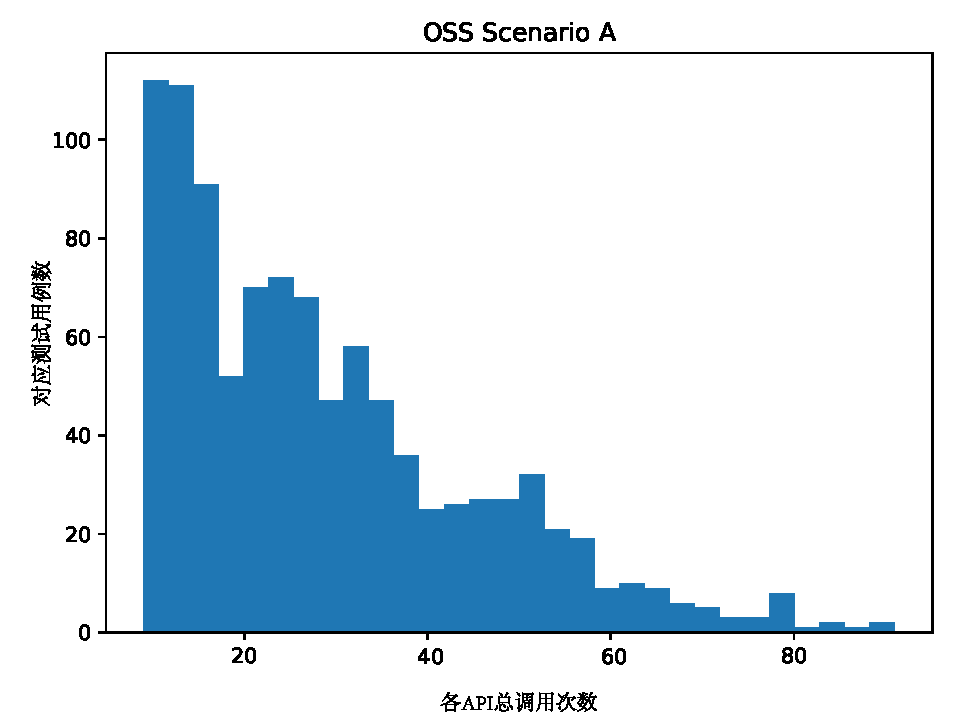
\includegraphics[width=200pt]{OSS_A_APICalls_cn.pdf}
                    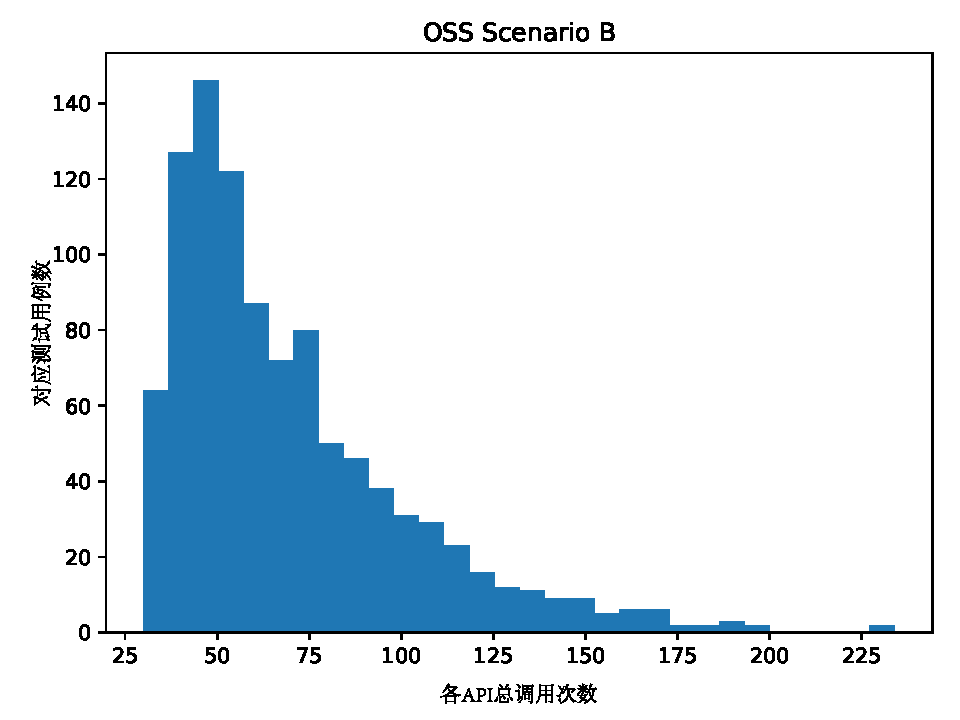
\includegraphics[width=200pt]{OSS_B_APICalls_cn.pdf}
                    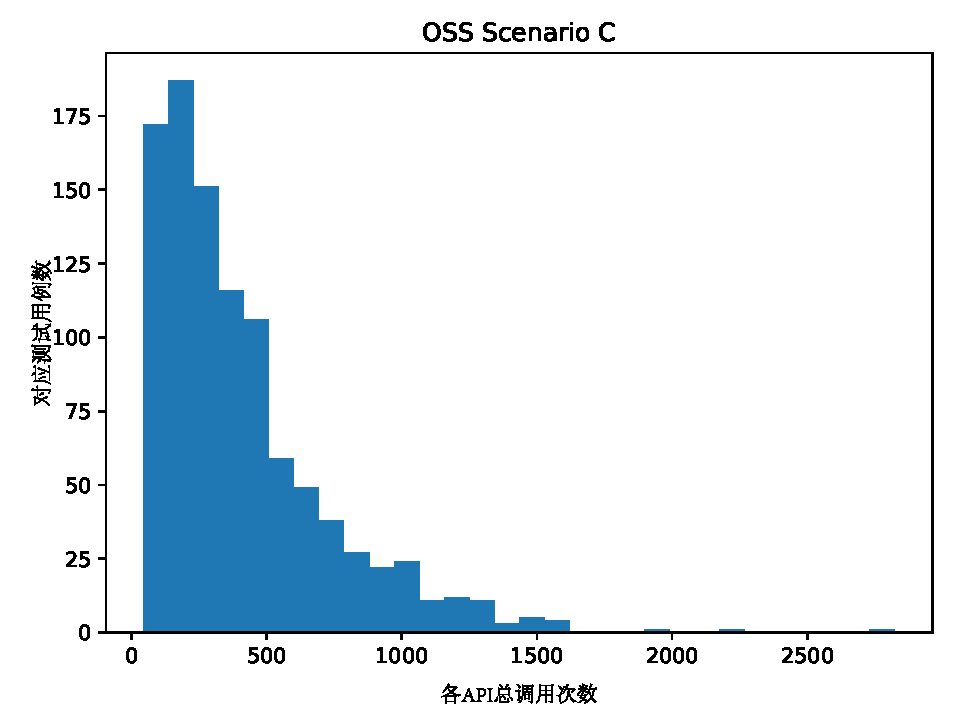
\includegraphics[width=200pt]{OSS_C_APICalls_cn.pdf}
                \end{minipage}
                \begin{minipage}{0.5\textwidth}
                    \centering
                    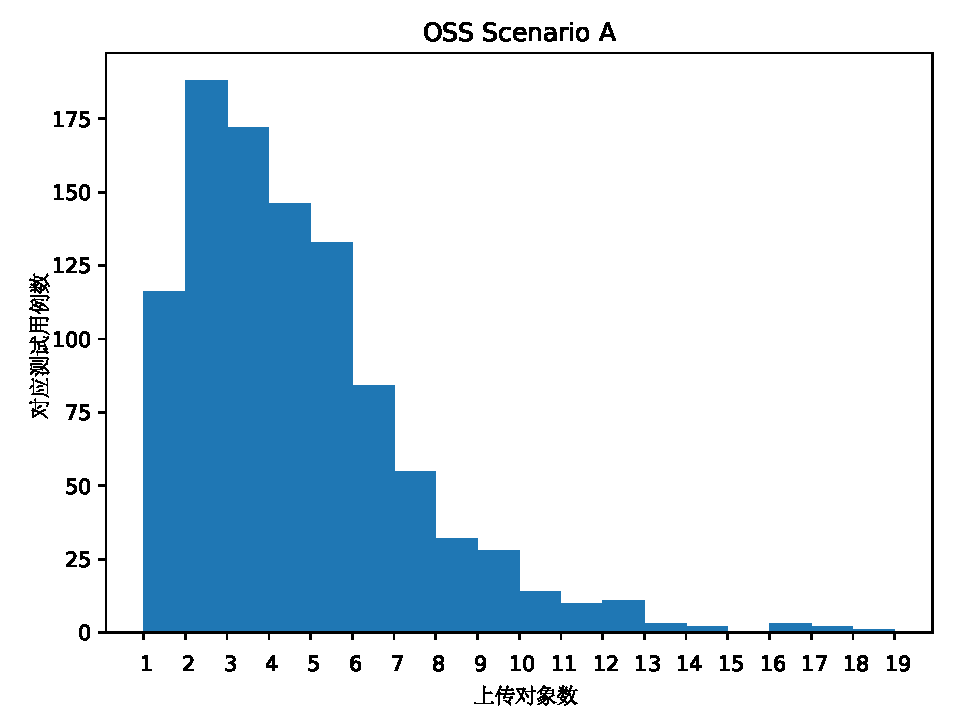
\includegraphics[width=200pt]{OSS_A_UploadedObj_cn.pdf}
                    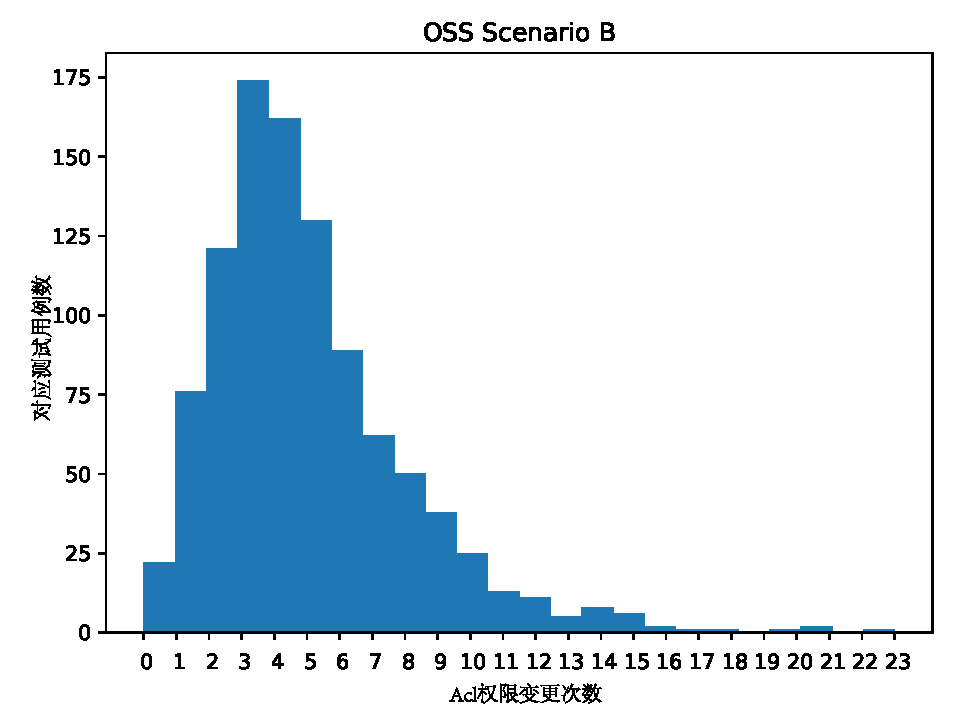
\includegraphics[width=200pt]{OSS_B_AclChange_cn.pdf}
                    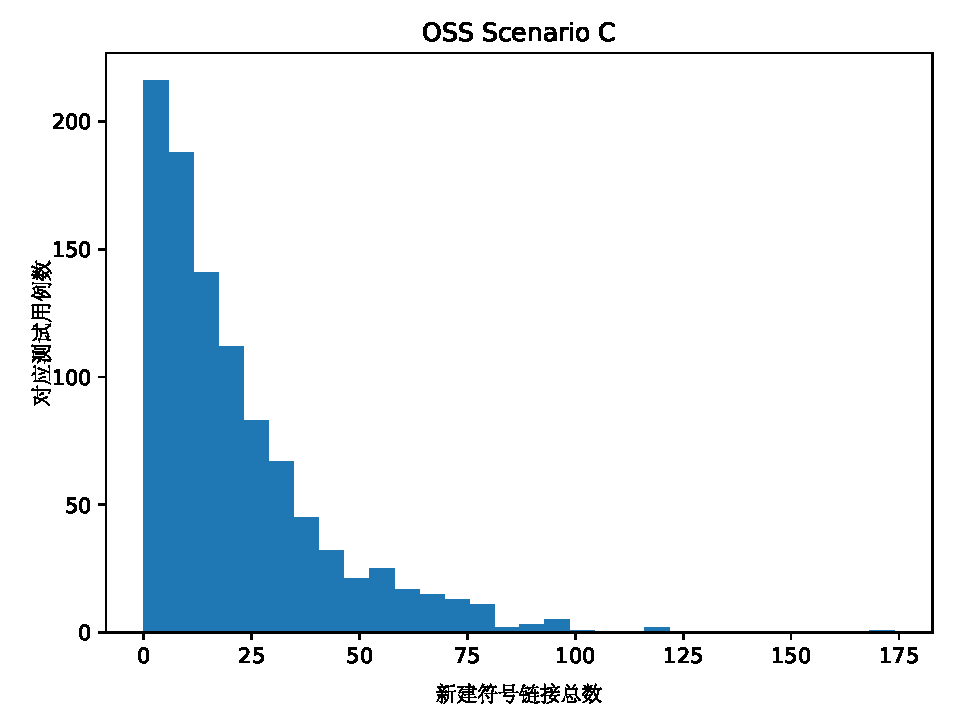
\includegraphics[width=200pt]{OSS_C_Putsymlink_cn.pdf}
                \end{minipage}
                \caption{OSS测试用例操作次数分布直方图. 基于Scenario A, Scenario B, Scenario C三个场景生成的1,000个测试用例. 左侧为每个测试用例调用API总次数分布直方图, 右侧为对每个场景选取一种典型API, 其调用次数的分布直方图.}
                \label{fig:OSS_stat}
            \end{figure}
            
            \begin{figure}[!htb]
                \centering
                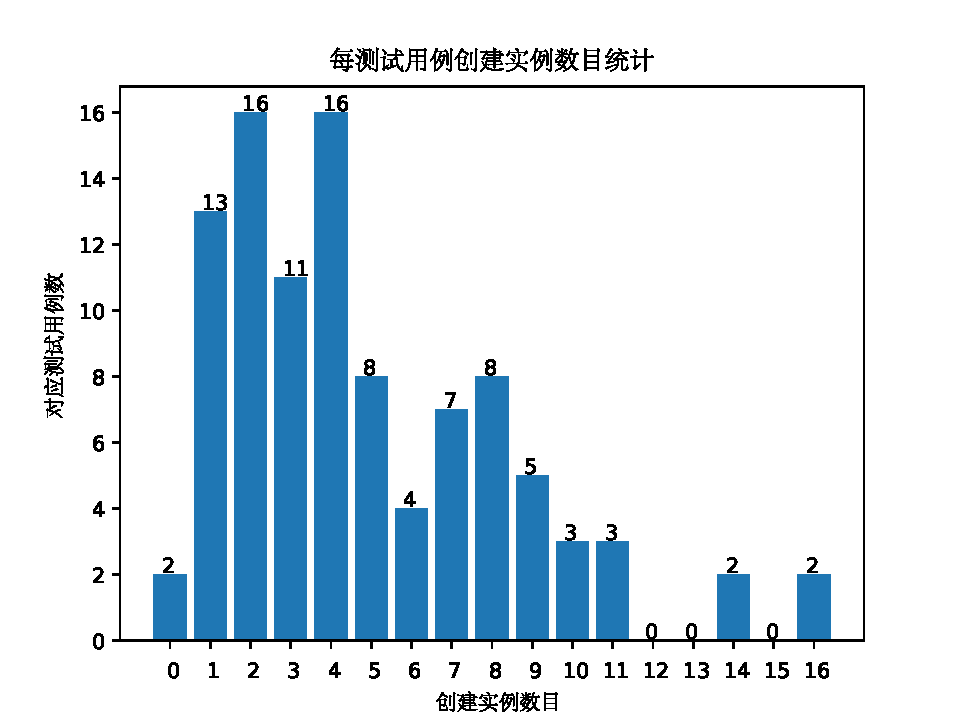
\includegraphics[width=200pt]{EC_instance_distribution_cn.pdf}
                \caption{ECS测试用例实例创建数分布直方图. 基于ECS测试场景生成的100个测试用例.}
                \label{fig:ECS_stat}
            \end{figure}
            
            在web API测试中, 测试用例的多样性可以通过很多不同的指标反映出来. 图\ref{fig:OSS_stat}反映了对于OSS服务, 生成的测试用例的总API调用次数和典型单API调用次数的统计分布情况. 图\ref{fig:ECS_stat}反映了对于ECS服务, 生成的测试用例创建的实例数的统计分布情况. 虽然由于不同API在场景中所处位置不同的原因, 每幅直方图中的分布区间差异较大, 但是整体分布模式是类似的, 即无论是API总调用数目, 单API调用数目, 还是实例创建数目, 分布均较分散. 这反映了生成的测试用例的多样性.
            
            值得注意的是, 虽然这些直方图反映的分布都与指数分布较为接近, 但这只是因为, 在这些场景中大致模式均为一个总状态连接到调用各API的分状态, 并拥有不为零的终止概率, 因此测试用例中各API的调用次数才近似于指数分布. 对于其他场景模式, 其余分布模式当然是完全可能出现的.
            
            测试用例的多样性主要归因于场景模型的概率性质, 在确定初始状态, 选择转移边, 以及确定是否终止等决策上, 场景模型均具有概率性质. 因此使用它生成的测试用例具有多样性的特征. 这是固定执行序列或普通测试脚本生成的测试用例所不具备的优势.

        \subsection{测试覆盖率}
            覆盖率是软件测试中的一项重要指标. 覆盖率有许多类型. 在本文使用的规约导向的黑盒API测试中, 无法获取源代码. 因此, 基于源代码的代码覆盖率指标和分支覆盖率指标无法使用. 本文评估时使用的覆盖率指标主要为API覆盖率和数据分区组合覆盖率.
            
            \subsubsection{API覆盖率}
            
                本文中, 定义某个API的覆盖率为, 在所有生成的测试用例中, 覆盖了这个API的测试用例个数与测试用例总数的比例. 在OSS系统的实验中, 对每个场景模型包含的API服务均计算了API覆盖率. 其中, Scenario B和Scenario C场景的API覆盖率十分理想. 除了“DeleteBucketLogging”这项API只被57.1\%的测试用例覆盖外, 所有其他API的覆盖率均超过了90\%.
                
                然而, 在Scenario A中, “DeleteBucketWebsite”, “DeleteMultipleObject”和“DeleteBucket”的API覆盖率均不足20\%, 尤其是“DeleteBucketWebsite”的覆盖率为0. 仔细研究这个现象后, 发现这是被测系统的一个故障引起的: 在请求了“PutBucketWebsite”之后, 对于其他关于对象和网页设置的API请求, 被测系统变得极易崩溃. 特别是, 在请求了“PutBucketWebsite”之后, 请求“GetBucketWebsite”一定会导致系统崩溃. 但是, 在场景中如果要经过与“DeleteBucketWebsite”关联的状态, 则一定会在之前经过与“GetBucketWebsite”关联的状态, 而在请求“GetBucketWebsite”之前又一定会请求“PutBucketWebsite”. 因此, 在到达与“DeleteBucketWebsite”关联的状态之前, 被测系统已经崩溃, 测试用例的执行已经结束. 自然无法覆盖“DeleteBucketWebsite”这项API了. 其余覆盖率较低的API也是类似原因. 实际上, 在Scenario A中一共只有8.5\%的测试用例是正常结束的, 而在无崩溃现象的Scenario B和Scenario C中所有测试用例均能正常结束.
                
                以上实验结果表明, 本文提出的场景模型和测试方法, 在OSS服务中可以有效覆盖被测系统的各个API接口. 另外, 某一API的异常低覆盖率很大程度上可以表征被测系统具有故障.
            
            \subsubsection{数据分区组合覆盖率}
            
                \label{sec:partition}
                
                组合测试策略\cite{grindal2005combination}是一种根据组合策略, 对测试的不同输入参数进行组合, 来生成测试用例的方法.
                
                在E-payment服务中, 实时贷记业务的API接口具有多达20个参数. 每个参数的可能取值, 包括合法取值与非法取值, 可以被划分为一些互不相交的集合, 即数据分区. 本文对E-payment服务测试时, 共考虑了其中13个参数的数据组合, 把每个参数的取值集合划分为2-5个分区,  它们的全组合共有1,152,000种. 评估指标为数据分区组合覆盖率, 即生成的测试用例覆盖的数据分区组合占总组合个数的百分比. 此覆盖率越高, 数据分区的组合被覆盖得越全, 测试效果越好. 
                
                本文提出了一种进行组合测试的场景模型模式, 详见附录\ref{sec:epayment_scenario_model}. 在此模式中, 每个非最末状态进行基于数据分区的单参数生成, 最末状态组合之前的单参数, 对被测系统发送请求. 使用此模式, 便可在本文的场景模型上运用组合测试策略.
                
                \begin{figure}[!htb]
                    \centering
                    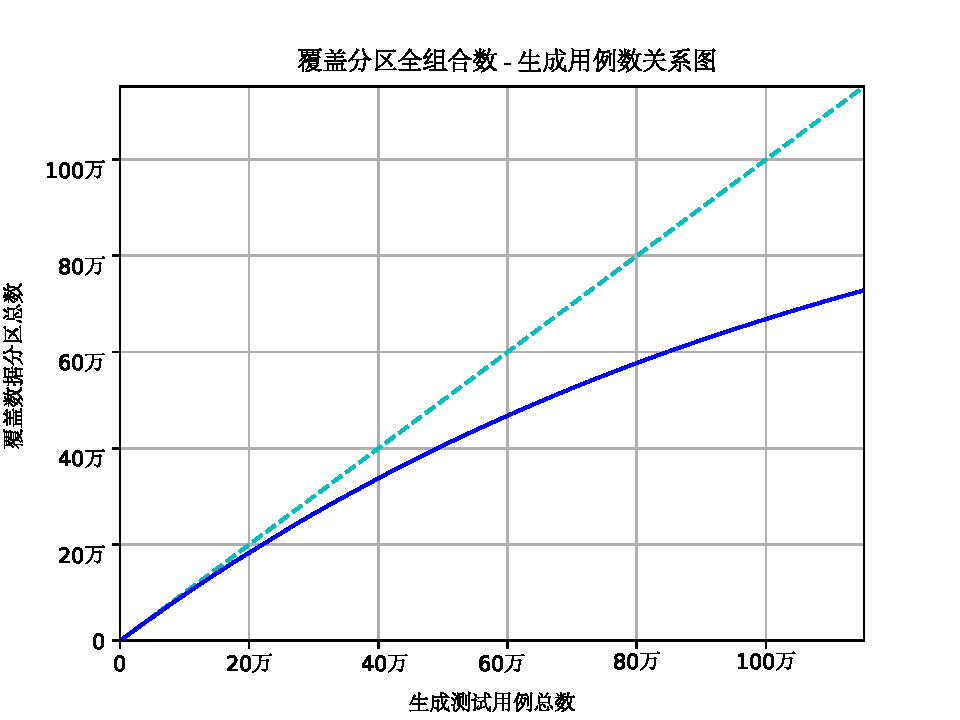
\includegraphics[width=200pt]{webank1_cn.pdf}
                    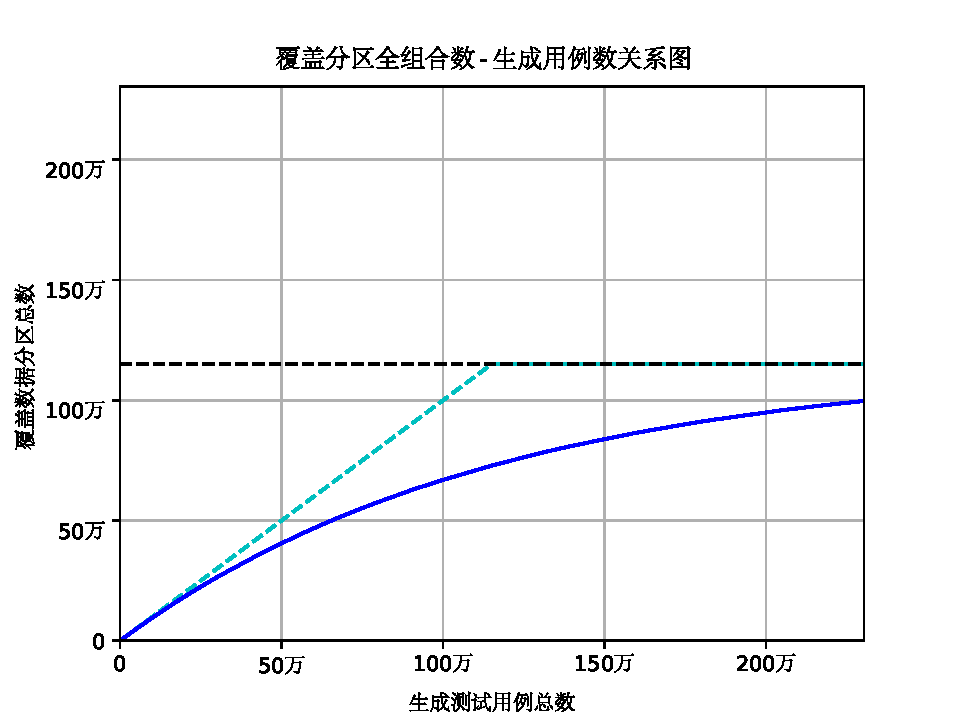
\includegraphics[width=200pt]{webank2_cn.pdf}
                    \caption{测试分区数 - 生成用例数关系图. 图中, 实线表示实验结果; 青色虚线为$y=x$, 表示最理想情况, 即每个测试用例覆盖一个新数据分区; 黑色虚线表示数据分区总数(1,152,000). 两幅子图系同一实验, 仅绘图尺度不同.}
                    \label{fig:partition}
                \end{figure}
                
                实验共生成了逾200万个测试用例, 图\ref{fig:partition}反映了生成的测试用例数目与它们覆盖的分区组合数目之间的关系. 在图中, 青色虚线表示最理想的测试用例生成方法, 即每个新生成的测试用例均覆盖一个新的数据分区; 黑色虚线表示数据分区的总数(1,152,000); 蓝色实线表示在本文的场景模型上运行组合测试策略的实验结果. 两幅子图采用了不同尺度, 左图反映测试用例数目不超过数据分区数目时的趋势, 右图则反映测试用例数目不超过数据分区数目\textbf{两倍}时的趋势.
                
                当生成的测试用例数为总数据分区组合数(1,152,000)时, 覆盖的数据分区组合数为728,239, 数据分区组合覆盖率为63.2\%. 当测试用例数为总数据分区组合数的两倍时, 覆盖数增加至996,642, 对应覆盖率为86.5\%. 此结果说明, 使用本文的场景模型实现组合测试策略时, 如果生成测试用例数与总数据分区组合数为同一数量级, 测试用例便可以覆盖大部分数据组合分区, 因此是十分有效的. 理论推导亦可验证此结论(详见附录\ref{sec:partition_deduction}).
    
        \subsection{故障检测能力}
        
            软件测试中, 一项基本的任务便是发现被测系统的故障与错误. 一个有实际应用价值的测试方法应能有效检测出系统故障.
            
            \begin{table}[!htb]
                \centering
                \begin{tabular}{lc}
                    \toprule
                    类型 & 占比 \\
                    \midrule
                    未写明的参数约束 & 15\% \\
                    未进行的输入检查 & 10\% \\
                    功能实现不完全 & 25\% \\
                    功能实现错误 & 5\% \\
                    被忽略的参数 & 5\% \\
                    不符合格式定义的响应 & 15\% \\
                    致命错误, 系统崩溃 & 25\% \\
                    \bottomrule
                \end{tabular}
                \caption{OSS系统中被检测出的故障的分类. 此表说明, 各种类型的故障均可以被本文的测试方法自动有效检出.}
                \label{tab:oss_bug_classification}
            \end{table}
            
            在OSS系统的实验中, 根据自动化生成的测试用例的反馈结果, 本工作成功发现并确认了20个系统的真实故障. 故障的具体分类见表\ref{tab:oss_bug_classification}. 其中, 65\%的故障是在编写简单场景验证API基本行为时发现的, 35\%的故障是在三个综合场景中发现的.
            
            而在来自工业界的ECS服务上, 实验生成的100个测试用例则检测出了以下异常与故障:
            \begin{itemize}
                \item 对于删除实例(“DeleteInstance”)的API请求, 依照文档描述, 只要当前实例处于停止状态, 操作即可成功. 但是, 实际测试发现, 当实例已经处于停止状态几秒钟后, 此请求仍然失败并返回403状态码. 由于几秒钟的延迟较小, 人工测试难以发现, 可能是此故障遗留至今的原因.
                
                \item 实例的状态域有许多中间的过渡态没有在API文档中描述. API文档只记录了“Running”和“Stopped”态, 实际上还有“Creating”, “Starting”和“Stopping”这些过渡状态.
                
                \item 停止实例(“StopInstance”)的API行为不稳定. 当“ForceStop”参数设定为真时, 正常情况下, 几秒钟内实例即被停止, 并对用户发出响应, 但是, 偶尔, 此操作需要数分钟时间完成, 从而导致测试用例抛出响应超时异常.
                
                \item 绝大多数情况下, 创建实例(“CreateInstance”)的API响应时间在1秒以内, 但是, 偶尔, 响应时间需约10秒, 从而导致测试用例抛出响应超时异常.
            \end{itemize}
            
            以上实验结果表明, 本文的场景模型和自动化测试方法可以有效检出系统的故障和错误, 具有实际应用价值.
    
        \subsection{测试效率}
    
            进行自动化测试的一项重要初衷, 便是提高测试效率, 节省人工时间成本. 本工作用实验和量化分析粗略地分析了本文测试方法的测试效率.
            
            随着如OpenAPI的API行为规范描述语言的快速发展和流行, 在接口设计阶段提供公开的Web API描述脚本变得越来越常见. 因此, 在软件测试阶段, 使用本文的方法, 只需要设计场景模型并编写场景脚本即可.
            
            \begin{table}[!htb]
                \centering
                \small
                \begin{tabular}{ccc|ccc|c}
                    \toprule
                    \multirow{2}{*}{场景} & 场景脚本 & \multirow{2}{*}{总耗时} & 估计对应     & 估计用例   & 估计     & 估计时间  \\
                                          & 大小     &                         & 测试用例个数 & 脚本总大小 & 人工耗时 & 节省率 \\
                    \midrule
                    Scenario A & 9.1 KB & 4.55 h & 4 & 12 KB & 6 h & 24.17\% \\
                    Scenario B & 9.6 KB & 4.80 h & 5 & 15 KB & 7.5 h & 36.00\% \\
                    Scenario C & 15.3 KB & 7.65 h & 8 & 24 KB & 12 h & 36.25\% \\
                    \bottomrule
                \end{tabular}
                \caption{OSS服务三个综合测试场景的耗时估计以及与人工方法耗时(估)的对比.}
                \label{tab:efficiency_esti}
            \end{table}
            
            在覆盖的功能点意义上, 每个场景模型可以等价于多个手工编写的测试用例. 以OSS服务的三个综合场景Sceanrio A、 Scenario B和Scenario C为例, 根据功能点等价的原则, 本实验对每个测试场景等价的手工测试用例数进行了较准确的估算. 另外, 如果人工编写测试脚本描述测试用例, 需要一定量的代码处理被测系统的启动/终止, 以及一定量的代码处理网络协议, 因此估计测试脚本的平均大小至少为3KB(约80行). 然后, 假设对于有经验的测试人员, 每2KB(约50行)代码的编写和调试时间为1小时. 有了这些数据, 即可估算自动化测试方法与人工测试方法所需的人工总耗时, 估算结果见表\ref{tab:efficiency_esti}.
            
            从表\ref{tab:efficiency_esti}中可以看出, 相比人工测试, 本文提出的自动化测试方法的效率提高直接反映在需要手工编写的脚本大小的减少, 这个减少在24\%到37\%之间. 此外, 正如\ref{sec:scenario_gui_edit}小节的讨论, 在可视化编辑工具的支持下, 测试场景模型的设计可通过类似拖拽绘制有向图的方法绘制出来, 然后自动生成场景描述脚本. 这很可能进一步显著提高自动化测试的效率. 总而言之, 根据以上科学估计, 可以得知, 使用本文的自动化测试方法可以有效节省人工时间成本, 提高测试效率.
